\documentclass[conference]{IEEEtran}
%\IEEEoverridecommandlockouts
% The preceding line is only needed to identify funding in the first footnote. If that is unneeded, please comment it out.
\usepackage{cite}
\usepackage{amsmath,amssymb,amsfonts}
\usepackage{algorithmic}
\usepackage{graphicx}
\usepackage{textcomp}
\usepackage{xcolor}
\usepackage{url}
\usepackage{graphicx}
\usepackage{subfig}
\usepackage{subcaption}

\def\BibTeX{{\rm B\kern-.05em{\sc i\kern-.025em b}\kern-.08em
    T\kern-.1667em\lower.7ex\hbox{E}\kern-.125emX}}
\begin{document}

\title{UrduVoiceCommand: End-to-End Automatic Voice Command Recognizer for Urdu Language using Deep Neural Networks}

\author{\IEEEauthorblockN{Mehreen Alam}
\IEEEauthorblockA{\textit{Computer Science Deparment} \\
\textit{National University of Computer and Emerging Sciences}\\
Islamabad, Pakistan \\
mehreen.alam@nu.edu.pk}
}

\maketitle

\begin{abstract}
The domain of Automatic Speech Recognition (ASR) has shown a phenomenal growth since the onset of deep learning techniques. Such techniques help build a complete end to end systems that are scalable, generic and understand the complexities inherent in audio representation of a language. The research area of Voice Commands Recognition for Urdu language is still untapped despite Urdu being used by over 100 million people across the globe. We build UrduVoiceCommand, the first ever Urdu Voice Command Recognition for desktop systems which frees the user from manually performing tasks like opening a folder, opening a search engine on a browser, or merely adjusting the brightness. Such features make the usability of the desktop systems easier and more friendly. We have used a three layer deep neural network and also added batch normalization, relu activation function and dropout, fine-tuning their optimal parameters after rigorous experimentation. We also developed a corpus of 1000 Urdu voice commands which mapped several variations of one voice command onto its corresponding operating system command. Our model gives a very encouraging results and sets the state-of-the-art accuracy to 55\%. It is the first attempt in this research area and shall open up avenues of further research in building Urdu Voice Command Recognition systems.
\end{abstract}

\begin{IEEEkeywords}
automatic speech recognition, continuous speech recognition, Urdu language, voice interface, deep neural networks
\end{IEEEkeywords}

\section{Introduction} \label{introduction}

Deep neural networks have become immensely popular because unparalleled performance in many of the research areas being worked on today. Computer vision \cite{goodfellow2016deep}, speech recognition \cite{deng2013new} and natural language processing \cite{young2018recent} are few areas that have taken a significant jump since the onset of deep learning techniques. To the best of our knowledge, no promising work has been done to apply deep learning techniques for any of the variety of automatic speech recognition tasks in Urdu language. Conventional methods are used which suffer from lack of generality, limited scalability, manual annotation and reliance on hand-crafted feature extraction. \\
`
Automatic Speech Recognition is a captivating research area today. Despite being worked on by researchers for the past many decades, many challenges still have to be addressed. This is primarily because of the complex nature of a natural language further complicated by taking the audio representation. In ASR, continuous speech is mapped onto a sequence of words. The main challenges of ASR are as follows:
\begin{itemize}
  \item Humans understanding of speech is based on learning and exposure to a wide range of vocabulary and language complexities over a long period of time. It is difficult to find such training environment to train any such model.
	\item Spoken language is much simpler to convey the message across than the written language since it has additional features like tones, expressions, pitch and volume to name a new.
	\item In addition to speech, humans communicate simultaneously using additional features like eye movement and postures to convery their point.
	\item Humans can decipher what is being said even with high levels of background noise.	
	\item Continuous speech recognition is even more challenging as there is no mapping of an audio sequence to a sequence of words and there remains the ambiguity of word boundary.
	\item ASR is sensitive to speaker's variability  which includes gender, age, tone, accent, speed of delivery to name a few.
	\item Two sentences spoken by the same person, in the same environment and in the same tone can vary which is unlike the written sentences where a sentence written any time is always the same.
\end{itemize}  
 
\begin{figure}[h!]
%\vspace{0.5cm}figure-UrduArchitecture
  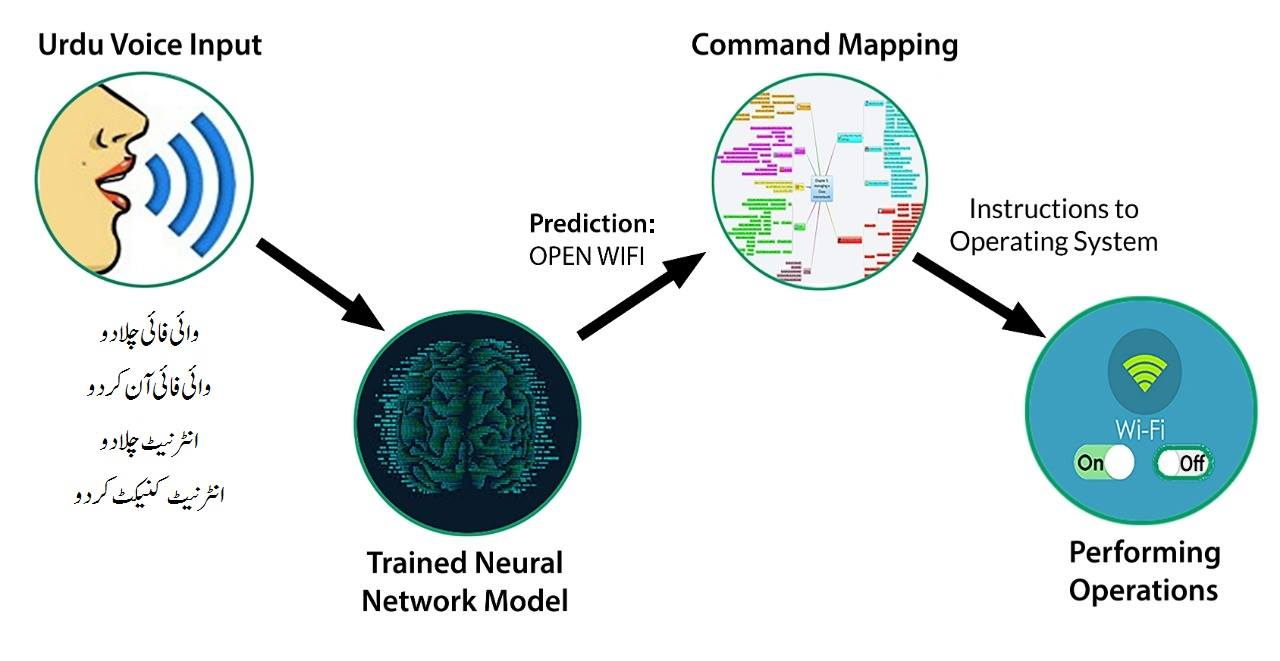
\includegraphics[width=\linewidth]{figure-UrduArchitecture.jpg}
  \caption{High Level Architecure of our proposed Model}
  \label{fig:figure-UrduArchitecture}
\end{figure} 

Out of the numerous tasks of ASR for Urdu language, we pick the research problem of mapping Urdu voice commands to the corresponding operating system commands. We chose a total of 12 commands and got around 80 different versions on the same command uttered in different ways by different people in different environments. However, we are not taking into consideration the noisy audio commands. Our model essentially takes as input an audio command, maps it onto one of the 12 voice commands chosen which is passed onto the operating system that then executes the command and the action is performed as shown in fig.\ref{fig:figure-UrduArchitecture}. We use three layer deep neural network to train the model that maps voice commands to any of the twelve classes of operating system commands. The operating system we have used for your work is Linux, but this can be extended to any operating system by simply changing the operating system specific commands.  

In the remainder of this paper, we will introduce the key ideas behind our speech recognition system. We give a review of related work in deep learning, end-to-end speech recognition and scalability in Section \ref{RelatedWork}. In Section \ref{Methodology}, we discuss in detail the dataset creation strategy, the model architecture and the methodology followed. We conclude with our experimental results demonstrating the state-of-the-art performance of UrduVoiceCommand in Section \ref{Results}, followed by a conclusions and future work in Section \ref{ConclusionsandFutureWork}.


\section{Related Work} \label{RelatedWork}

For the past two decades, feed forward neural network models have been explored to address the research area of automatic speech recognition \cite{bourlard2012connectionist}. Many enhancements have been done in basic neural network modeling techniques, most prominent ones are use of recurrent neural networks and convolutional neural networks \cite{robinson1996use,sainath2013deep}. Due to its immense boost in performance, use of deep learning has become almost inevitable in any of the speech recognition problems \cite{mohamed2012acoustic,hinton2012deep,dahl2012context,jaitly2012application}. Most significantly, deep learning combined with Convolutional Neural Networks and Recurrent Neural Networks are known to set state-of-the-art \cite{abdel2012applying} and \cite{graves2013speech}. 

Since deep learning techniques are data-driven, presence of a large-scale dataset which is representative of the problem target is essential to get good results \cite{HannunCCCDEPSSCN14}. Crowd-sourcing and data augmentation are one of the most widely used techniques to increase the scale of the data and also to add variability to it \cite{1315150,sainath2013deep,HannunCCCDEPSSCN14}.
Specifically, there is hardly any worth-mentioning voice command system for Urdu language using latest techniques like deep learning. \cite{7571287} attempt to address the asr research problem for Urdu by using Hidden Markov Model. \cite{ali2015automatic} tries to apply asr to Urdu digits recognition using support vector machines, linear discriminant analysis classifier and random forest. \cite{raza2018rapid} makes a voice speech corpus which is yet to be used for an application.

To the best of our knowledge, our work is the first attempt to come up with a Voice Command model for Urdu language using modern techniques from deep learning.


\section{Methodology}\label{Methodology}
\subsection{Dataset}\label{Dataset}
Since there was no publicly available dataset available, we had to generate the dataset ourselves. Using crowd-sourcing techniques, we were able to generate 1000 voice commands in Urdu language. The data was kept balanced and for all the 12 total voice commands classes almost 80 voice commands were generated. Heterogeneity and variations were the key factors kept in mind and the 80 variations of the voice commands were generated by 10 different people all belonging to different age groups with equal representation from both the genders. Since the factor of noise is out of the scope of our work, recordings were done in a quite place. Twelve commands that were targeted are mentioned in table \ref{table:totalVoiceCommands}. The variations with which these commands were asked are listed out in detail in fig. \ref{tableTotalVoiceCommandsVariations}. We refer to this corpus as Dataset1.

\begin{table}[h!]
  \begin{center}
    \caption{Voice Commands}
    \label{table:totalVoiceCommands}
    \begin{tabular}{l|l}
      \hline
			Wifi On & Wifi Off\\
			Bluetooth On & Bluetooth Off\\
			Brightness High & Brightness Low\\
			Volume Up & Volume Down\\
			Volume Mute & Open Google\\
			Power Off & Restart\\
			\hline
    \end{tabular}
  \end{center}
\end{table}

For the sake of experimentation, we also merged the classes in groups of 2 on the basis of the operation they invoke. For examples. WiFi On and Wifi Off are merged to one class of WiFi. Brightness High and Brightness Low are merged to one class of Brightness. We refer to this corpus as Dataset2.

\begin{figure}[h!]
  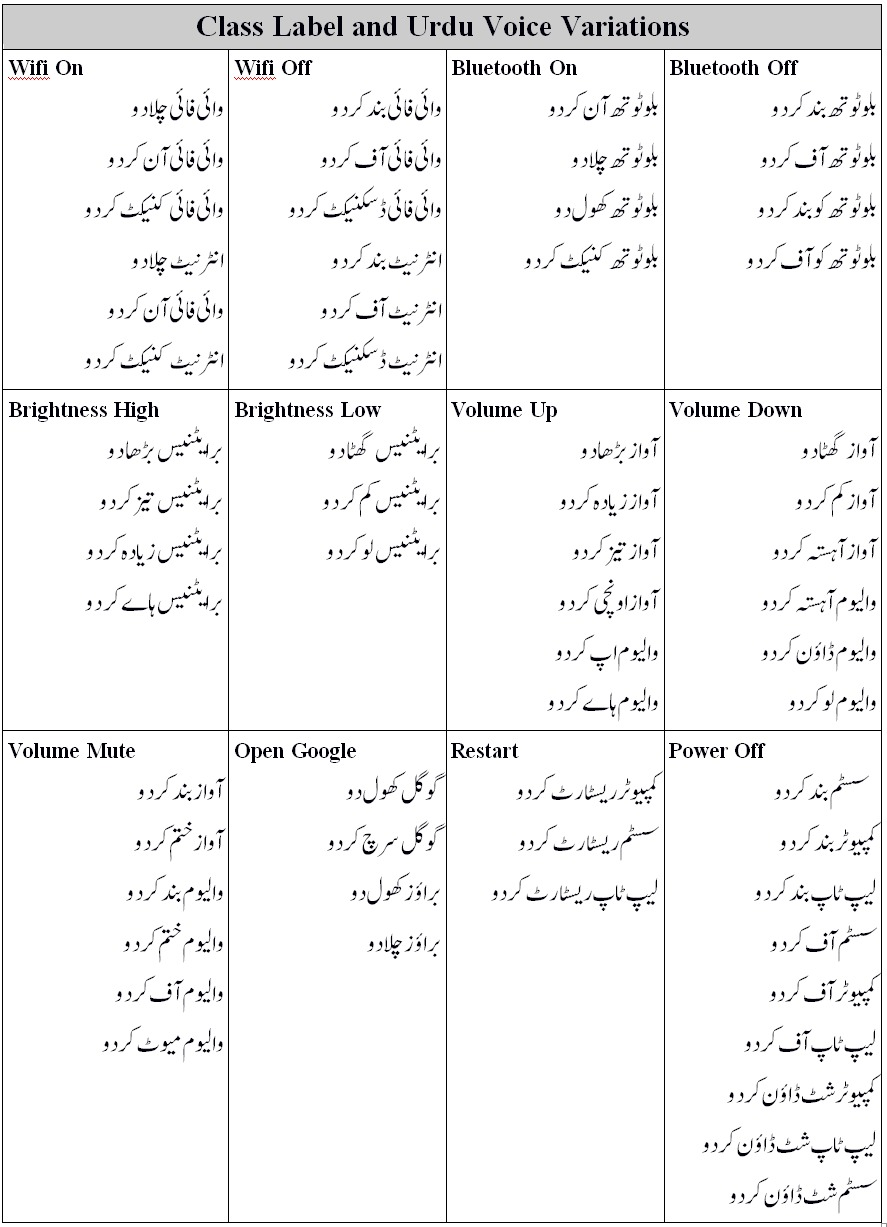
\includegraphics[width=\linewidth]{tableTotalVoiceCommandsVariations.jpg}
  \caption{Voice Command Variations for every Command Class}
  \label{tableTotalVoiceCommandsVariations}
\end{figure} 

\subsection{Model Architecture}
After rigorous and thorough experimentation, we came up with our model which is a feed forward deep neural network with total depth of three. We have used batch normalization for all the three layers. ReLU activation function is used for first two layers and softmax at the last layer for categorizing the output in one of the twelve classes. DropOut was also used as a regularization mechanism at the second layer with valee of 0.25. We are using a total of 128 neurons in the second layer. Details are shown in fig.\ref{figure-modelArchitecture}. We used Adam as our optimizer with epsilon = 1*10-7 and learning rate of 0.0001 which is gradually reduced by a factor of 10 as the model converges. We divided our data in the ratio of 75:15:15 for training, validation and testing purposes respectively.

\begin{figure}[h!]
  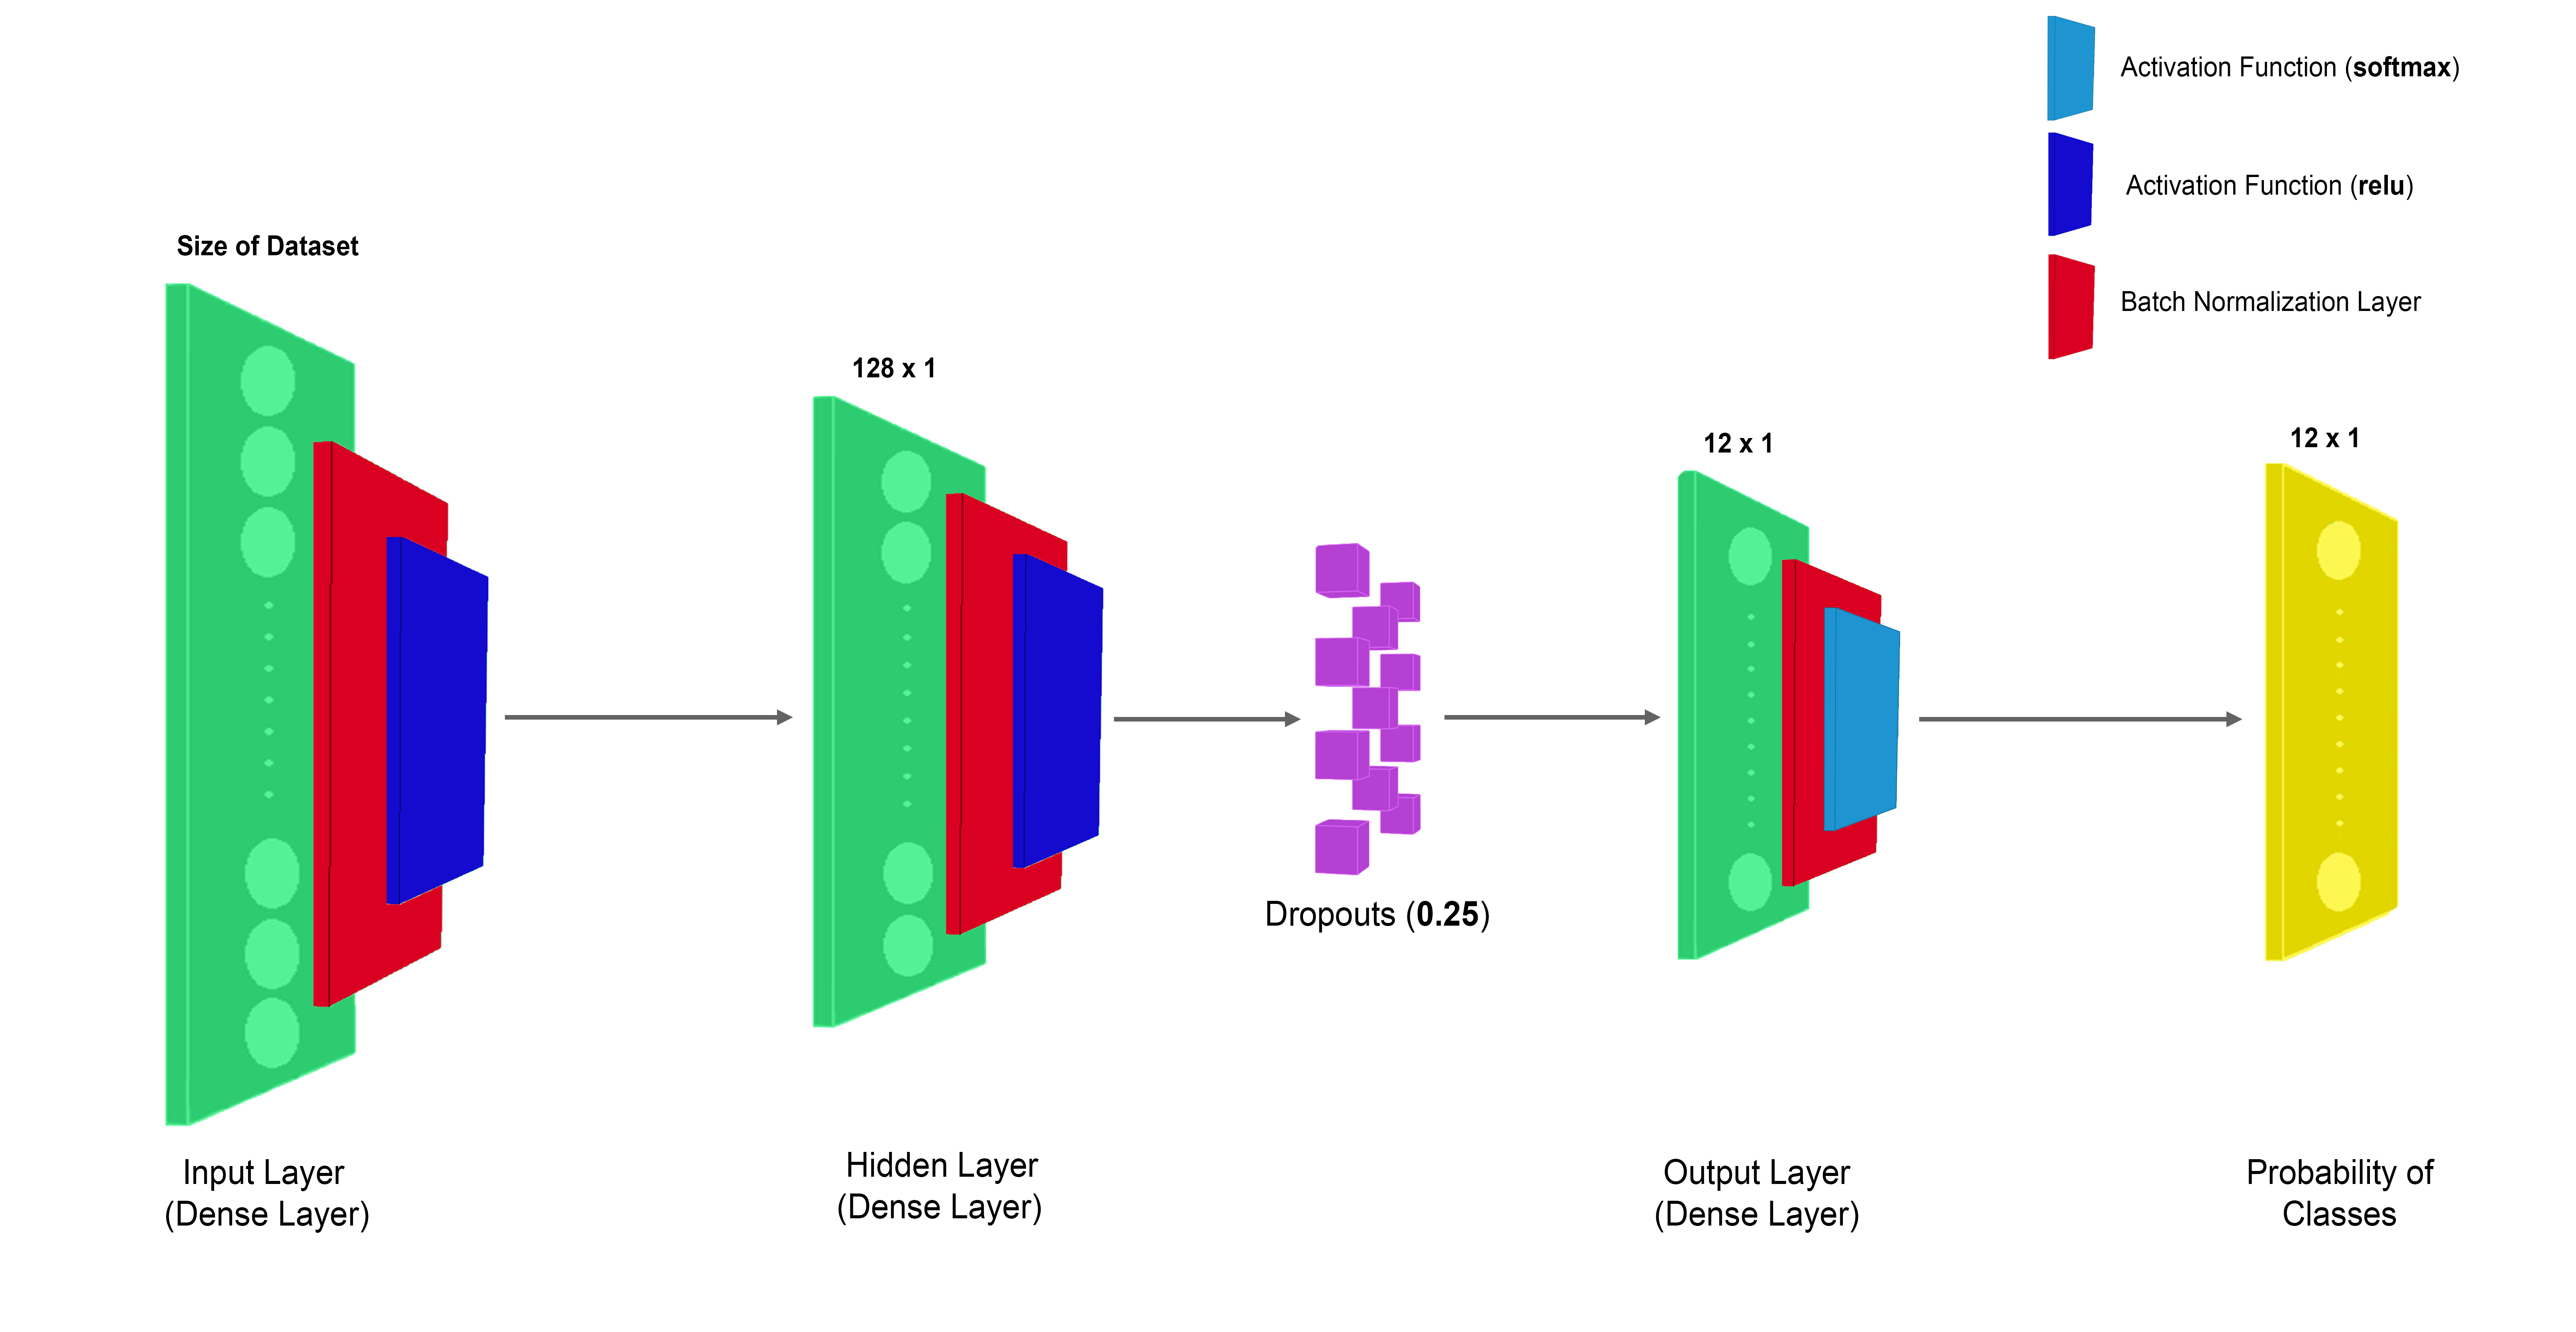
\includegraphics[width=\linewidth]{figure-modelArchitecture.png}
  \caption{Detailed Model Architecture}
  \label{figure-modelArchitecture}
\end{figure} 

\subsection{Methodology}
Voice command is directly fed to our model without any pre-processing done separately. We extract both the temporal and spectral audio features as amplitude vs. time signal. The temporal features are extracted from the time domain, such as energy of signal, zero crossing rate etc, whereas, the spectral features are extracted from the frequency domain, by converting the time based signal into the frequency domain using the Fourier Transform, such as MFCCs, Mel-spectrogram, spectral centroid, contrast, flux etc. For our model, we use the following ten features: mfcc, chroma\_stft,  chroma\_cqt, chroma\_cens, melspectrogram, mfcc, rmse, spectral\_centroid, spectral\_bandwidth, spectral\_contrast, spectral\_flatness, spectral\_rolloff, poly\_features, tonnetz, zero\_crossing\_rate.\\

These audio features are then used for our feed forward deep neural network model and model is trained rigorously until the model converges. Inputs are mapped to exactly one voice command, (e.g. Open WiFi), which has the maximum probability out of the total of 12 voice commands. Once the class is determined, it can be used to issue the particular command on the any operating system. For experimentation purposes, we have used Linux as it is an open-source operating system with no administrative restrictions.

\begin{figure}[h!]
\caption{Spectograms of Voice Commands of four sample commands.}
\label{table:spectograms}
\centering
\subfloat[Volume Up]{
  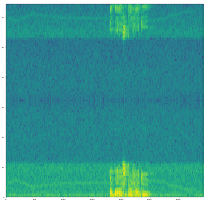
\includegraphics[width=35mm]{VolumeUp.png}
}
\subfloat[Volume Down]{
  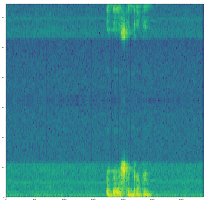
\includegraphics[width=35mm]{VolumeDown.png}
}
\newline
\subfloat[Brightness High]{
  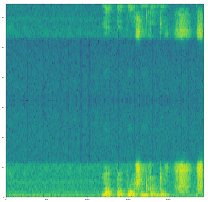
\includegraphics[width=35mm]{BrightnessHigh.png}
}
\subfloat[Brightness Low]{
  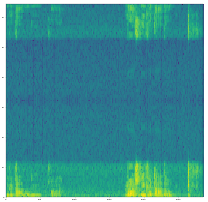
\includegraphics[width=35mm]{BrightnessLow.png}
}
\end{figure}


\section{Results}\label{Results}
After thorough experimentation, our model gives several useful and interesting results. Firstly, it gives 55 \% accuracy on the test set of the complete dataset, Dataset1, which is very encouraging as it is very hard to get such accuracy on continuous speech recognition task as show in table \ref{table:datasetAccuracy}. Secondly, our model gave accuracy of 76\% on the test set on Dataset2 which has merged representation of similar classes as mentioned in Section \ref{Dataset}. There is such a huge difference of almost 1.5 times in the results of both the datasets because of the difficulty model faces to distinguish between two similar classes, ie WiFi on and WiFi as compared to two totally different commands like WiFi On and Brighness ON. We can also judge the likelihood of such a phenomenon by looking at the spectrogram of the all the classes as shown in fig.
 \ref{table:spectograms}. 

\begin{table}[h!]
  \begin{center}
    \caption{Accuracy on Both the Datasets}
    \label{table:datasetAccuracy}
    \begin{tabular}{S|S}
      \hline
      \textbf{Dataset} & \textbf{Accuracy}\\
      \hline
      Dataset1 & 55\%\\
      Dataset2 & 76\%\\
			\hline
    \end{tabular}
  \end{center}
\end{table}

Overall, it was motivating to see that the model has accurately absorbed and understood the audio complexities inherent in the language Urdu. Continuous speech recognition has its own challenges which were aptly covered by our system. Specifically, our speech recognition successfully covers the challenge of limited vocabulary and limited grammatical structures to learn from. Model's learning simply relied in audio input only, unlike the real world scenario where humans communicate via various features like eye movement, postures, etc. Though very minimal, our model is resistant to any background noise.
  

We are very excited to present the first ever deep neural network based voice command system for Urdu language and the first corpus of 1000 Urdu Voice Commands. 

\section{Conclusions and Future Work} \label{ConclusionsandFutureWork}
It is very motivating to see our systems setting the state-of-the-art for Voice Command Recognition system in Urdu language for desktop systems. To the best of our knowledge, any effort done in this regard uses conventional techniques like HMM and decision trees and no attempt has been made to address this research problem using deep learning techniques. Our system is generic, scalable and caters to the complexities of the natural language. 
We plan to further our work by covering broader range of commands and applying more sophisticated deeper models. 


\begin{thebibliography}{00}
%\begin{thebibliography}{6}

\bibitem {bourlard2012connectionist}
Bourlard, Herve A and Morgan, Nelson, "`Connectionist speech recognition: a hybrid approach,"' Springer Science \& Business Media. 247, 2013
  
\bibitem {renals1994connectionist}
Renals, Steve and Morgan, Nelson,et al., "`Connectionist probability estimators in HMM speech recognition,"' IEEE Transactions on Speech and Audio Processing, vol. 2, pp. 161-174, 1994

\bibitem {sainath2013deep}
Sainath, Tara N and Mohamed, Abdel-rahman and Kingsbury, Brian and Ramabhadran, Bhuvana, "`Deep convolutional neural networks for LVCSR,"' IEEE international conference on Acoustics, speech and signal processing (ICASSP), 2013

\bibitem {robinson1996use}
Robinson, Tony and Hochberg, Mike and Renals, Steve, "`The use of recurrent neural networks in continuous speech recognition,"'  Automatic speech and speaker recognition,pp. 233-258, 1996

\bibitem {mohamed2012acoustic} 
Mohamed, Abdel-rahman and Dahl, George E and Hinton, Geoffrey, et al, "`Acoustic modeling using deep belief networks,"' IEEE Trans. Audio, Speech \& Language Processing. vol. 20, pp. 14-22, 2012

\bibitem {hinton2012deep} 
Hinton, Geoffrey and Deng, Li and et al, "`Deep neural networks for acoustic modeling in speech recognition: The shared views of four research groups,"' IEEE Signal processing magazine. vol. 29, pp. 82-97,  2012

\bibitem {dahl2012context}
Dahl, George E and Yu, Dong and Deng, Li and Acero, Alex, "`Context-dependent pre-trained deep neural networks for large-vocabulary speech recognition,"' IEEE Transactions on audio, speech, and language processing. vol. 20, pp. 30-42, 2012

\bibitem {jaitly2012application}
Jaitly, Navdeep and Nguyen, Patrick and Senior, Andrew and Vanhoucke, Vincent, "`Application of pretrained deep neural networks to large vocabulary speech recognition,"' Thirteenth Annual Conference of the International Speech Communication Association, 2012

\bibitem {abdel2012applying}
Abdel-Hamid, Ossama and Mohamed, Abdel-rahman and Jiang, Hui and Penn, Gerald, "`Applying convolutional neural networks concepts to hybrid NN-HMM model for speech recognition,"' IEEE International Conference on Acoustics, Speech and Signal Processing (ICASSP),2012

\bibitem {graves2013speech}
Graves, Alex and Mohamed, Abdel-rahman and Hinton, Geoffrey, "`Speech recognition with deep recurrent neural networks,"' IEEE International Conference on Acoustics, Speech and Signal Processing (icassp), 2013.

\bibitem {sak2014long}
Sak, Ha{\c{s}}im and Senior, Andrew and Beaufays, Fran{\c{c}}oise, "`Long short-term memory recurrent neural network architectures for large scale acoustic modeling,"' Fifteenth annual conference of the international speech communication association, 2014.

\bibitem {7178838}
T. N. Sainath and O. Vinyals and A. Senior and H. Sak, "`Convolutional, Long Short-Term Memory, fully connected Deep Neural Networks,"' IEEE International Conference on Acoustics, Speech and Signal Processing (ICASSP)}, 2015.

\bibitem {HannunCCCDEPSSCN14}
Awni Y. Hannun, Carl Case, Jared Casper, et al, "`Deep Speech: Scaling up end-to-end speech recognition,"' CoRR, 2014.

\bibitem {1315150} 
Y. LeCun and Fu Jie Huang and L. Bottou, "`Learning methods for generic object recognition with invariance to pose and lighting,"' Proceedings of the 2004 IEEE Computer Society Conference on Computer Vision and Pattern Recognition, 2004.

\bibitem {7571287}
Asadullah and A. Shaukat and H. Ali and U. Akram, "`Automatic Urdu Speech Recognition using Hidden Markov Model,"' International Conference on Image, Vision and Computing (ICIVC), 2016.

\bibitem {ali2015automatic}
Ali, Hazrat and Jianwei, An and Iqbal, Khalid, "`Automatic speech recognition of Urdu digits with optimal classification approach,"' International Journal of Computer Applications, vol. 118.

\bibitem {raza2018rapid}
Raza, Agha Ali and Athar, Awais and Randhawa, Shan and et al, "`Rapid Collection of Spontaneous Speech Corpora using Telephonic Community Forums,"' Proc. Interspeech, 2018.

\bibitem {young2018recent}
Young, Tom and Hazarika, Devamanyu and Poria, Soujanya and Cambria, Erik, "`Recent trends in deep learning based natural language processing,"' IEEE Computational intelligenCe magazine. vol. 13, 2018.

\bibitem {deng2013new}
Deng, Li and Hinton, Geoffrey and Kingsbury, Brian, "`New types of deep neural network learning for speech recognition and related applications: An overview,"` Acoustics, Speech and Signal Processing (ICASSP), 2013.

\bibitem {goodfellow2016deep}
Goodfellow, Ian and Bengio, Yoshua and Courville, Aaron and Bengio, Yoshua, "`Deep learning,"' 2016.


\end{thebibliography}
\end{document}
